% --------------------------------------------------------------------------- %
% Leaflet for  GOMTRAIC 2012      %
% --------------------------------------------------------------------------- %
% Created with Brian Amberg's LaTeX Poster Template, using the baposer class
% Please refer for the     %
% attached README.md file for the details how to compile with `pdflatex`.     %
% --------------------------------------------------------------------------- %
% $LastChangedDate:: 2011-09-11 10:57:12 +0200 (V, 11 szept. 2011)          $ %
% $LastChangedRevision:: 128                                                $ %
% $LastChangedBy:: rlegendi                                                 $ %
% $Id:: poster.tex 128 2011-09-11 08:57:12Z rlegendi                        $ %
% --------------------------------------------------------------------------- %
\documentclass[a4paper,portrait,fontscale=0.65]{baposter}

\usepackage{relsize}		% For \smaller
\usepackage{url}			% For \url
\usepackage{epstopdf}	% Included EPS files automatically converted to PDF to include with pdflatex
\usepackage{graphicx}
%%% Global Settings %%%%%%%%%%%%%%%%%%%%%%%%%%%%%%%%%%%%%%%%%%%%%%%%%%%%%%%%%%%

\graphicspath{{pix/}}	% Root directory of the pictures 
\tracingstats=2			% Enabled LaTeX logging with conditionals

%%% Color Definitions %%%%%%%%%%%%%%%%%%%%%%%%%%%%%%%%%%%%%%%%%%%%%%%%%%%%%%%%%

\definecolor{bordercol}{RGB}{0,0,0}
\definecolor{headercol1}{RGB}{186,215,230}
\definecolor{headercol2}{RGB}{80,80,80}
\definecolor{white}{RGB}{255,255,255}
\definecolor{boxcolor}{RGB}{186,215,230}
\definecolor{darkgray}{RGB}{68,68,71}
\definecolor{brightgreen}{RGB}{111,248,71}
\definecolor{blue}{RGB}{102,163,253}
\definecolor{darkblue}{RGB}{43,92,125}
\definecolor{leftgray}{RGB}{101,117,107}
\definecolor{backgray}{RGB}{47,48,53}
%%%%%%%%%%%%%%%%%%%%%%%%%%%%%%%%%%%%%%%%%%%%%%%%%%%%%%%%%%%%%%%%%%%%%%%%%%%%%%%%
%%% Utility functions %%%%%%%%%%%%%%%%%%%%%%%%%%%%%%%%%%%%%%%%%%%%%%%%%%%%%%%%%%

%%% Save space in lists. Use this after the opening of the list %%%%%%%%%%%%%%%%
\newcommand{\compresslist}{
	\setlength{\itemsep}{1pt}
	\setlength{\parskip}{0pt}
	\setlength{\parsep}{0pt}
}

%%%%%%%%%%%%%%%%%%%%%%%%%%%%%%%%%%%%%%%%%%%%%%%%%%%%%%%%%%%%%%%%%%%%%%%%%%%%%%%
%%% Document Start %%%%%%%%%%%%%%%%%%%%%%%%%%%%%%%%%%%%%%%%%%%%%%%%%%%%%%%%%%%%
%%%%%%%%%%%%%%%%%%%%%%%%%%%%%%%%%%%%%%%%%%%%%%%%%%%%%%%%%%%%%%%%%%%%%%%%%%%%%%%

\begin{document}
\typeout{Poster rendering started}

%%% Setting Background Image %%%%%%%%%%%%%%%%%%%%%%%%%%%%%%%%%%%%%%%%%%%%%%%%%%
% \background{
% 	\begin{tikzpicture}[remember picture,overlay]%
% 	\draw (current page.north west)+(-2em,2em) node[anchor=north west]
% 	{\includegraphics[height=1.1\textheight]{background}};
% 	\end{tikzpicture}
% }

%%% General Poster Settings %%%%%%%%%%%%%%%%%%%%%%%%%%%%%%%%%%%%%%%%%%%%%%%%%%%
%%%%%% Eye Catcher, Title, Authors and University Images %%%%%%%%%%%%%%%%%%%%%%
\begin{poster}{
	grid=false,
        columns=2,
	% Option is left on true though the eyecatcher is not used. The reason is
	% that we have a bit nicer looking title and author formatting in the headercol
	% this way
	eyecatcher=true, 
	borderColor=darkgray,
	headerColorOne=darkgray,
	headerColorTwo=black,
	headerFontColor=white,
	% Only simple background color used, no shading, so boxColorTwo isn't necessary
	boxColorOne=white,
	headershape=rounded,
	headerfont=\Large\sf\bf,
	textborder=rectangle,
        bgColorOne=darkblue,
        bgColorTwo=backgray,
	background=shadeTB,
	headerborder=open,
  boxshade=plain
}
%%% Eye Cacther %%%%%%%%%%%%%%%%%%%%%%%%%%%%%%%%%%%%%%%%%%%%%%%%%%%%%%%%%%%%%%%
{
  
\includegraphics[height=2cm]{golem}
}
%%% Title %%%%%%%%%%%%%%%%%%%%%%%%%%%%%%%%%%%%%%%%%%%%%%%%%%%%%%%%%%%%%%%%%%%%%
{
\textcolor{black}{\Huge\textbf{\textsc{GOMTRAIC}}}\vspace{0.5em}
}
%%% Authors %%%%%%%%%%%%%%%%%%%%%%%%%%%%%%%%%%%%%%%%%%%%%%%%%%%%%%%%%%%%%%%%%%%
{
 \textsc{GO}lem re\textsc{m}ote \textsc{trai}ning \textsc{C}ourse
}
%%% Logo %%%%%%%%%%%%%%%%%%%%%%%%%%%%%%%%%%%%%%%%%%%%%%%%%%%%%%%%%%%%%%%%%%%%%%
{
% The logos are compressed a bit into a simple box to make them smaller on the result
% (Wasn't able to find any bigger of them.)
% \setlength\fboxsep{0pt}
% \setlength\fboxrule{0.5pt}
% 	\fbox{
% 		\begin{minipage}{14em}
% 			\includegraphics[width=10em,height=4em]{colbud_logo}
% 			\includegraphics[width=4em,height=4em]{elte_logo} \\
% 			\includegraphics[width=10em,height=4em]{dynanets_logo}
% 			\includegraphics[width=4em,height=4em]{aitia_logo}
% 		\end{minipage}
% 	}

\includegraphics[height=2cm]{fjfi.png}
}

\headerbox{Do \textsc{YOU} want to}{name=motivation,column=0,row=0, span=2}{
  \begin{itemize}
  \item \textbf{\textsc{operate}} a real tokamak?
  \item \textbf{\textsc{experience}} fusion research?
  \item \textbf{\textsc{plan, perform}} and \textbf{\textsc{evaluate}} a ``high level'' experiment?
  \end{itemize}

}

\headerbox{Course Outline}{name=outline, column=0, below=motivation}{
  \begin{itemize}
  \item A course focused on basic understanding of experimental tokamak physics and control
  \item For undergraduate and postgraduate students interested in experimental tokamak physics
  \item Participants do not need to leave their country to get experienced in tokamak operation. They can participate even from their home
  \item \textsc{gomtraic} 2012 starts on March, 6th and finishes three months later, on May, 30th 2012
  \item Participants will address 9 tasks from basic tokamak physics and technology

  \end{itemize}
}

\headerbox{\textsc{golem} tokamak}{name=golem, column=1, below=motivation}{
The basis of \textsc{gomtraic} is remote operation of the \textsc{golem} tokamak, see \url{http://golem.fjfi.cvut.cz},  which is operated at the Czech  Technical University, Faculty of  Nuclear Sciences and Physical  Engineering in Prague
\begin{center}
  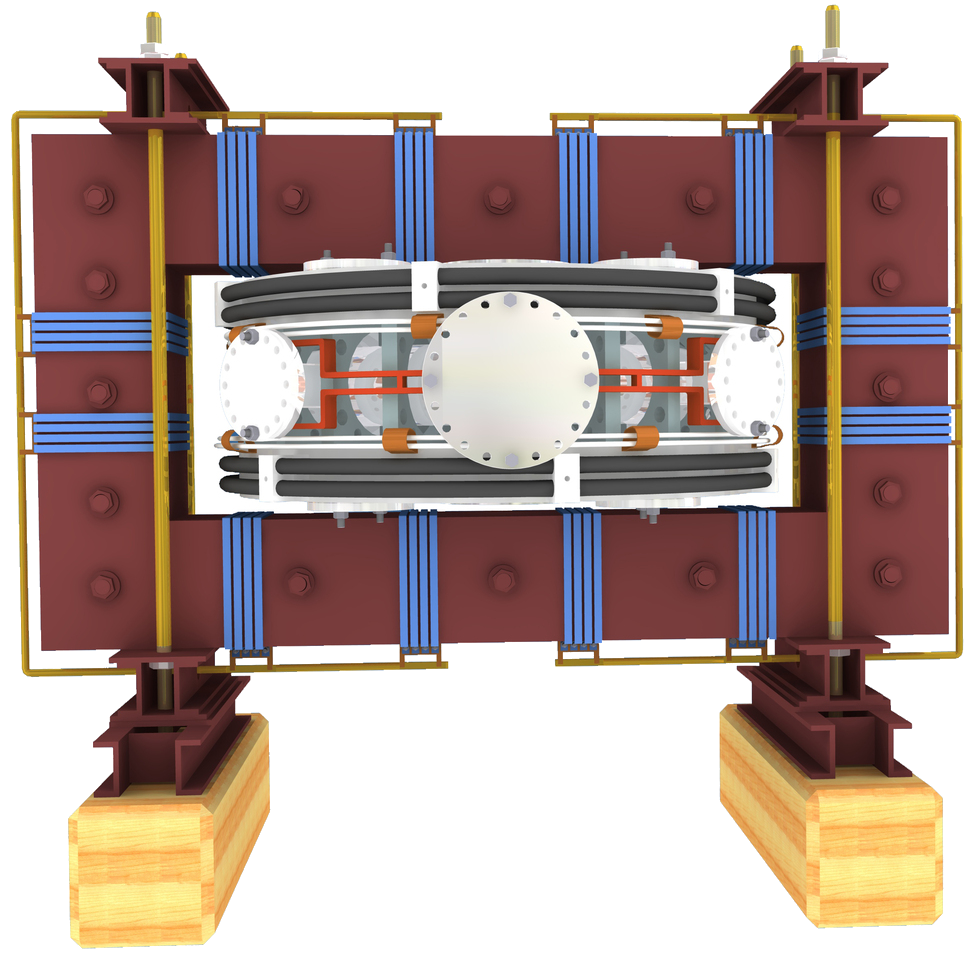
\includegraphics[width=.8\textwidth]{golem-model}
\end{center}
}

\headerbox{Acknowledgment}{name=acknowledgment, column=0,below=outline,  above=bottom}
{
  The course is supported by \textsc{Fusenet} and the Czech Technical university
}
\headerbox{References}{name=references, column=1, below=golem, above=bottom}
{
  \begin{itemize}
  \item \textsc{gomtraic} website \\ \url{http://gomtraic.fjfi.cvut.cz}
  \item \textsc{golem} tokamak website \\ \url{http://golem.fjfi.cvut.cz}
  \end{itemize}
}
\end{poster}
\end{document}
